\chapter{Beam dynamics}
This chapter is dedicated to introduce the basic Accelerator Physics concepts and the terminology required for this dissertation. For detailed discussions about the topics presented here, the author recommends the references~\cite{sands1970physics, wiedemann2007physics}.

After the storage ring coordinate system definition in the Section~\ref{coord}, the dynamics of a single electron will be described in the Sections~\ref{tranverse} and~\ref{longitudinal}. Then one can introduce the excitation and damping processes in the description and apply statistical methods to obtain equilibrium parameters for an ensemble of electrons -- the electron beam. This will be briefly done in the Section~\ref{equilibrium}. In the Section~\ref{perturbations} it is presented and discussed the perturbations on the beam dynamics, which are fundamental to this work.
\section{Coordinate System}\label{coord}
To describe the motion of electrons in a storage ring, a coordinate system definition is required and for this sake the concept of reference orbit is necessary. With proper initial conditions, an ideal electron (also called synchronous electron), which has the storage ring nominal energy $E_0$, will follow a closed orbit and this specific periodic path is defined as the reference orbit. The motion of an arbitrary electron is then described in terms of small deviations from the reference orbit, which is taken as the coordinate system origin. 

The dipoles are the elements of the magnetic lattice that defines the reference orbit that is curvilinear. Ideally, the dipoles deflects the electrons in just one direction (called radial or horizontal), therefore the ideal orbit defines an orbital plane in the storage ring. It is convenient to use a curvilinear and comoving coordinate system. The longitudinal axis $s$ can be defined as tangent to the local orbit, the horizontal $x$ is defined in the radial direction and the vertical $y$ is perpendicular to the orbital plane. A graphical representation of this coordinate system can be seen in Figure~\ref{syst}.
\begin{figure}
    \centering
    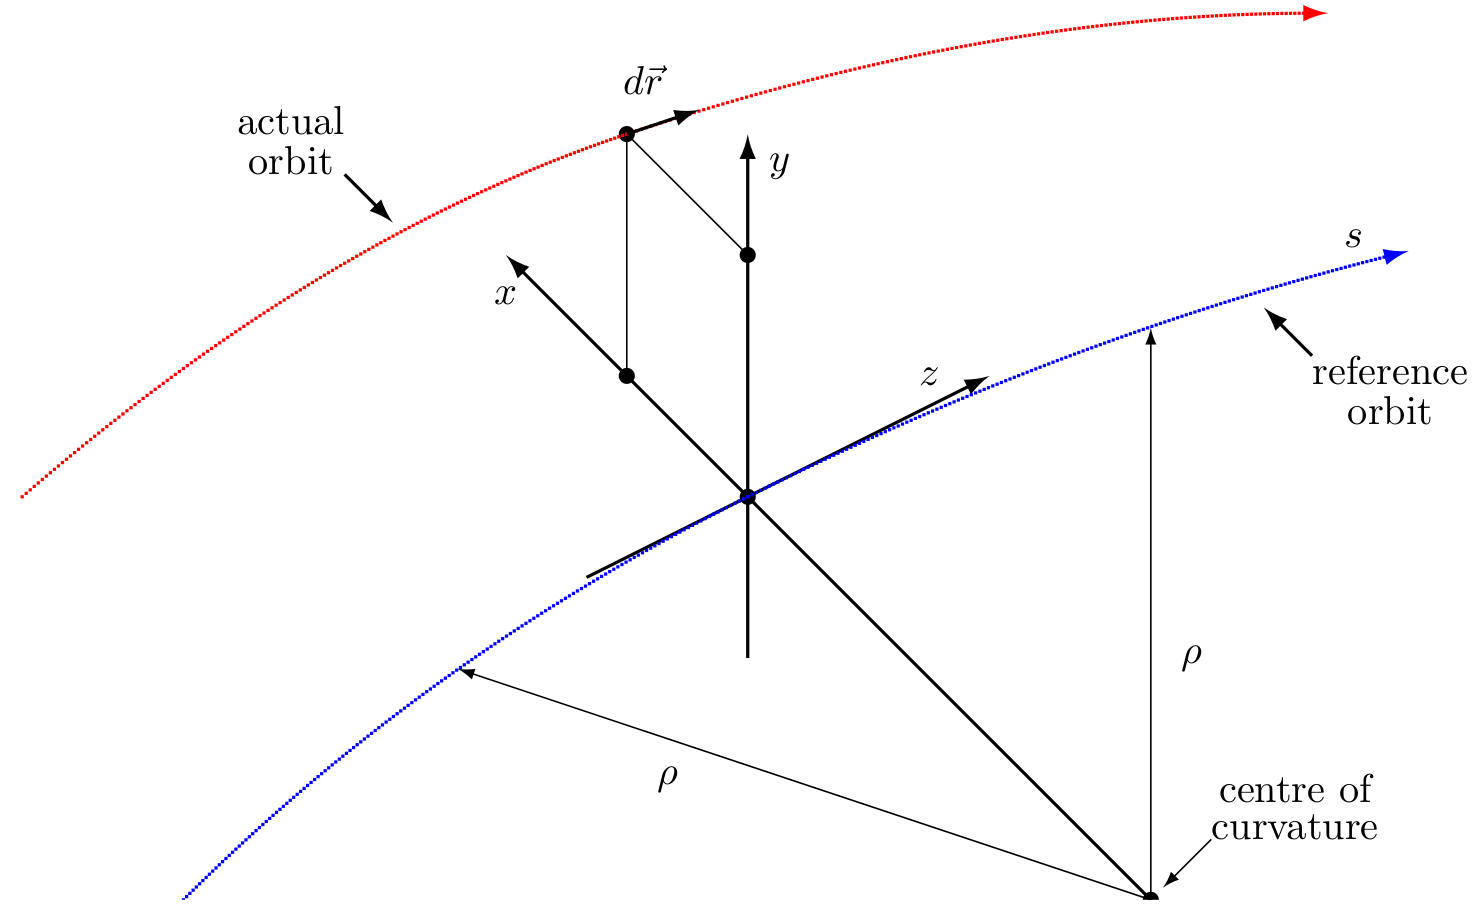
\includegraphics[scale=0.25]{figures/reference_system.png}
    % 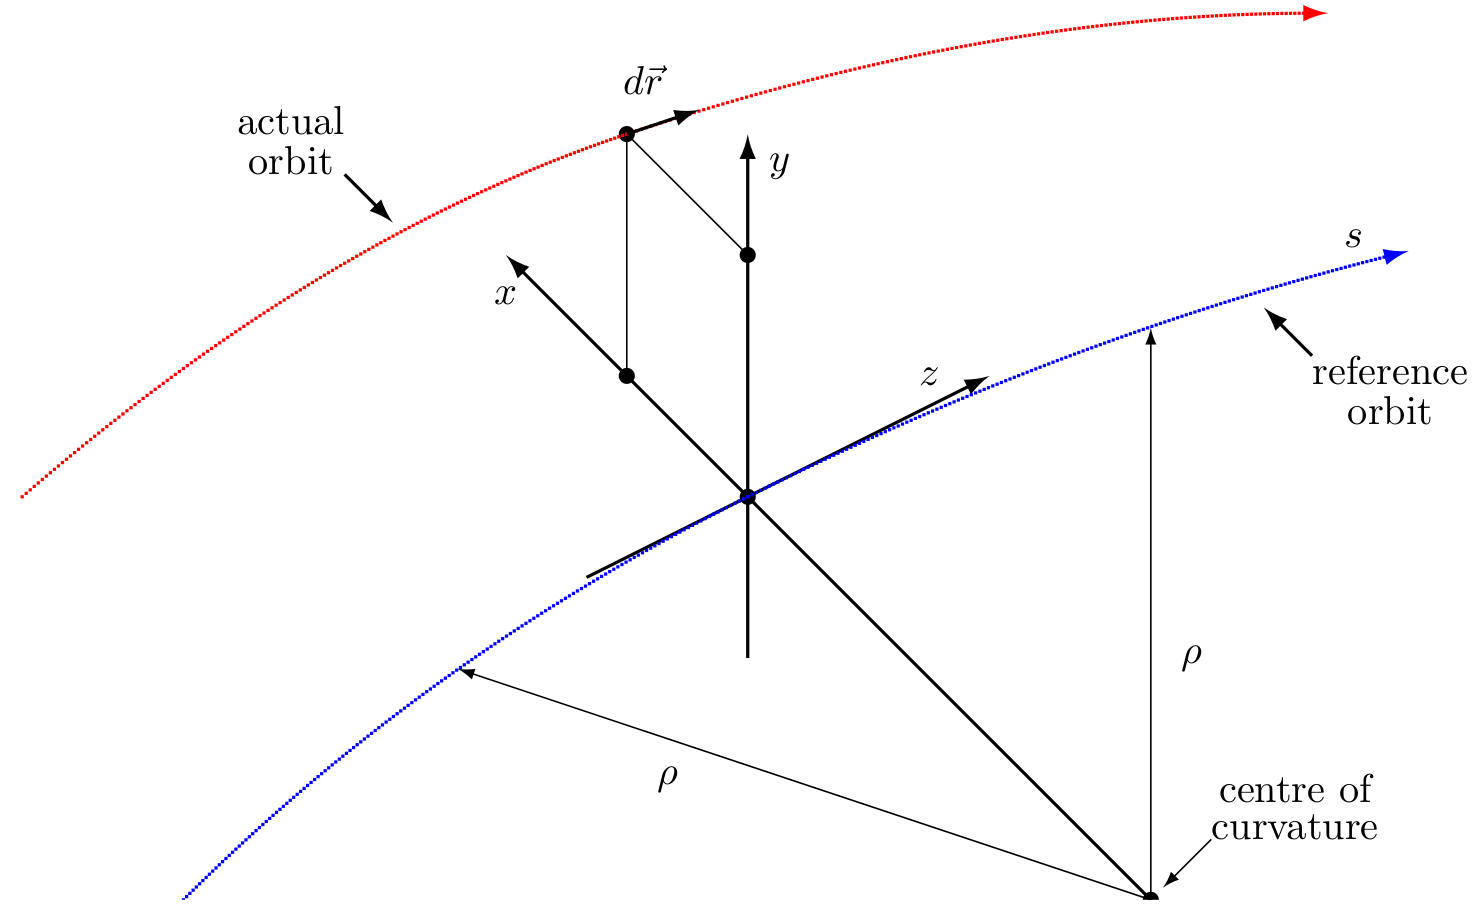
\includegraphics[width=\textwidth]{figures/reference_system.png}
    \caption{Coordinate system used in storage rings~\cite{madx}.}
    \label{syst}
\end{figure}

Electrons in a storage ring are in the ultra-relativistic regime, where $E \approx pc$ and the major contribution to the total momentum is longitudinal $p = \sqrt{p_s^2 + p_x^2 + p_y^2} \approx p_s$. It is assumed that transverse displacements $(x, y)$ of these electrons to the reference orbit are small, then the ratios $p_x/p$ and $p_y/p$ are small as well and they can be related to geometric quantities, namely angular deviations:
\begin{align*}
    x' &= \frac{\dif x}{\dif s} \approx \frac{p_x}{p}, \\
    y' &= \frac{\dif y}{\dif s} \approx \frac{p_y}{p}.
\end{align*}

The approximations made above are called paraxial. The coordinates $(x, x', y, y')$ defines a four dimensional (4D) phase space, where the transverse dynamics is described. Note that the displacements are functions of the longitudinal $s$ coordinate, replacing the time $t$ that is commonly used to describe the dynamics of a system. This substitution is convenient since the $s$ coordinate is periodic for a storage ring and the transverse coordinates derivatives can be interpreted geometrically.

To describe the longitudinal dynamics, one can define two more coordinates. The first is the difference of longitudinal position $s(t)$ of a generic electron relative to the position $s_{\mathrm{sync}}(t)$ of the synchronous electron:
\begin{equation}
    z(t) := s_{\mathrm{sync}}(t) - s(t).
\end{equation}

The variable $t$ represents the wall-clock time. The coordinate $z$ can be used in time units as well, represented by $\tau$ and the conversion is made by $\tau(t) = z(t)/c$. 

For the last coordinate it is used the electron relative energy deviation from the nominal energy, which is also typically small:
\begin{equation}
    \delta := \frac{E - E_0}{E_0}.
\end{equation}

Finally, $(x, x', y, y', z, \delta)$ defines a six dimensional (6D) phase space where the transverse and longitudinal dynamics of the electrons in a storage ring can be studied.
\section{Transverse Dynamics}\label{tranverse}
The transverse dynamics describes the motion of the electrons in the 4D phase space $(x, x', y, y')$. Assuming that the typical time scale in the longitudinal dynamics is much greater than the transverse time scale, the two dynamics can be treated independently. This is called the adiabatic approximation and is a good approximation to describe the transverse motion in storage rings. In Sirius storage ring, while it takes around 200 turns to the electrons perform one complete energy oscillation, in just one turn the same electrons realize 49 and 14 complete oscillations in $x$ and $y$ planes, respectively.

% In the present section the linear transverse dynamics for a single electron in a storage ring is reported and the next one concerns its longitudinal dynamics.
\subsection{Betatron Oscillations}
A simpler version of a magnetic lattice is composed by dipoles and quadrupoles only. The dipoles bends the electrons path around the ring and defines an ideal orbit. The dipole field can be seen as the zero-order expansion of the lattice magnetic fields. The next terms of the expansion are field gradients, mainly related to the quadrupoles. This setup composes the linear magnetic lattice, where the magnetic field expansion is up to first order.

Assuming this linear approximation and that the transverse directions are independent, i.e., there is no transverse coupling terms, the Hamiltonian of an electron in the storage ring is \footnote{The approximated transverse Hamiltonian is obtained from the Hamiltonian of a relativistic charged particle on magnetic fields: $H = q\phi + c\sqrt{m^2c^2 + \left(\vec{p} - q\vec{A}\right) }$.}:
\begin{equation}
    H \approx \dfrac{{x'}^2}{2} + \dfrac{{y'}^2}{2} + \left(K(s)- G^{2}(s)\right)\dfrac{{x}^2}{2} - K(s) \frac{y^2}{2} - G(s) x \delta.
    \label{transv_hamilton}
\end{equation}

$G(s)$ is called curvature function and $K(s)$ is the focusing function, with the following expressions:
\begin{align}
    G(s) &= \dfrac{1}{\rho(s)} = \dfrac{e}{p_0}B(s), \\
    K(s) &= \dfrac{e}{p_0}\left.\dfrac{\partial B(s)}{\partial x}\right|_{y=0},
\end{align}
where $p_0$ is the ideal electron momentum. The dipoles magnetic field $B(s)$ must in the vertical direction to deflect the electrons horizontally. Observe that the function $G(s)$ is the inverse of the radius of curvature of the electron path through the dipoles. $G(s)$ and $K(s)$ are defined by the magnetic lattice and they are called lattice functions. For a storage ring, these functions are periodic, i.e., $G(s) = G(s+L_0)$ and $K(s) = K(s+L_0)$, where $L_0$ is the storage ring circumference.

% The quantity $R = B(s)\rho(s) = \dfrac{p_0}{e} \approx \dfrac{E_0}{ec}$ is called magnetic rigidity and it is a property of the stored electron. For the Sirius storage ring the electron magnetic rigidity is approximately 10.

From the Hamiltonian in Eq.~\eqref{transv_hamilton}, the equations of motion are:
\begin{align}
    x'' + \left(K(s) - G^{2}(s)\right)x &= G(s) \delta, \\
    y'' - K(s)y &= 0.
\end{align}

From the adiabatic approximation, in this derivation it was considered that the energy deviation $\delta$ is constant during the transverse motion.

The equation of motion for the horizontal plane contains a non-homogeneous term $G(s)\delta$ due to the energy dispersion created at dipoles. This term couples the horizontal and longitudinal motions.

If we consider only the homogeneous part, the $x$ and $y$ equations can be cast in the same form:
\begin{equation}
u'' + K_u(s) u = 0,
\label{hill}
\end{equation}
where $u = x$ or $y$, $K_x(s) = K(s) - G^2(s)$ and $K_y(s) = -K(s)$. Note that $K_x \approx -K_y$ if we consider $G^2/K \ll 1$, which is a good approximation for strong-focusing magnetic lattices. This reflects the fact that a focusing quadrupole in $x$ plane is necessarily defocusing in the $y$ plane and vice-versa. 

The homogeneous Eq.~\eqref{hill} is called Hill equation, which is similar to a simple harmonic oscillator equation, except for the important fact that the term $K_u$ is $s-$dependent and periodic. The authors in~\cite{CourantSnyder1958} proposed a pseudo-harmonic solution for the Hill equation:
\begin{equation}
    u_{\beta}(s) = \sqrt{2 J_u \beta_u (s)} \cos \left(\varphi_u(s) - \phi_u\right).
    \label{eq:beta_oscillation}
\end{equation}

This solution describes the so-called betatron oscillations. $\beta_u(s)$ is called betatron function and $\varphi_u(s)$ is the betatron phase advance. Inserting this solution in the Hill equation, it is obtained that the $\beta_u(s)$ must satisfy the following differential equation:
\begin{equation}
    \dfrac{1}{2}\beta_u {\beta''_u} -  \left(\dfrac{\beta'_u}{2}\right)^2 + K_u(s) \beta^2_u = 1,
    \label{beta_equation}
\end{equation}
and also that the betatron function and phase advance are related by
\begin{equation}
\varphi_u(s) = \int_{0}^{s} \dfrac{1}{\beta_u(\bar{s})} \dif \bar{s}.
\end{equation}

In storage rings, the betatron function is a periodic solution for Eq.~\eqref{beta_equation}.

The parameters $J_u$ and $\phi_u$ are constants defined by the electron initial conditions. One can show that the constant $J_u$ is written in terms of $(u, u')$ by
\begin{equation}
    2J_u = \gamma_u u^2 + 2 \alpha_u u u' + \beta_u {u'}^2,
    \label{invariant}
\end{equation}
for every longitudinal position $s$ and using the identities $\alpha_u(s) = -\beta_u'(s)/2$ and $\gamma_u(s) = (1 + \alpha_u^2(s))/\beta_u(s)$. These three functions $\left\{\alpha_u(s), \beta_u(s), \gamma_u(s)\right\}$ are called Twiss functions and depends only on the magnetic lattice.

In the Eq.~\eqref{invariant} it is shown that, for each position $s$, the betatron oscillations performed by the electrons  in the storage ring over the turns draws a ellipse in the phase space $(u, u')$. Since the assumptions made so far allows us to consider the system as conservative, the Liouville theorem applies, therefore the area of this ellipse is invariant. From Eq.~\eqref{invariant}, the ellipse area is $A_u = 2 \pi J_u$, following that $J_u$ is a invariant of motion. It is also possible to obtain this result applying the canonical transformation of action-angle variables in the Hamiltonian~\eqref{transv_hamilton}, identifying the action with $J_u$ (in this case, it is an invariant by construction), and the phase variable with $\varphi_u$.

Once these concepts are presented, we define the particle emittance as $\varepsilon_u = 2J_u$. In this way, the particle emittance can be interpreted as the area of the ellipse that electron follows in the 4D phase space during betatron oscillations, divided by $\pi$:
\begin{equation}
    \varepsilon_u = \frac{A_u}{\pi}.
\end{equation}

As discussed, it follows that the particle emittance is a invariant for the betatron motion. From the ellipse equation analysis, the maximum values for $u$ and $u'$ are:
\begin{align}
    u_{\beta, \mathrm{max}}(s) &= \sqrt{\varepsilon_u \beta_u(s)}, \\
    {u}_{\beta, \mathrm{max}}'(s) &= \sqrt{\varepsilon_u \gamma_u(s)}.
\end{align}

In a storage ring, the betatron phase advance accumulated over one turn is related to the number of betatron oscillations realized by the electrons. This number is called the tune of the machine, given by
\begin{equation}
    \nu_u = \dfrac{1}{2\pi} \oint \dfrac{1}{\beta_u({s})} \dif {s},
\end{equation}
where the closed integral represents an integration where the lower limit is an arbitrary $s$ and the upper limit is $s + L_0$, closing one turn around the ring.

The tune has a integer part (the number of complete betatron oscillations over one turn) and a fractional part. Because of this fractional part the values of $(x, x', y, y')$ at some $s$ may be different for each turn. The betraton oscillations peaks and valleys are $\pm \sqrt{\varepsilon_u \beta_u(s)}$. Therefore, the emittance $\varepsilon_u$ and the $\beta_u(s)$ function defines the envelope of the betatron oscillations. The importance of the betatron function will be further discussed throughout this work.

The tune fractional part is closely related to resonances. If the fractional part is zero, i.e., the tune is an integer number, in every turn the particles will have the same coordinates $(u, u')$ for every $s$. Then if there are dipolar field errors at the magnetic lattice, these errors will distort the electrons orbit in the same way at every turn, increasing the distortion amplitude and leading to electron losses. If the fractional part is $1/2$, the resonance is excited by quadrupolar field errors. Generally, there are resonances that can be excited if the tunes satisfy the relation
\begin{equation}
    m \nu_x + n \nu_y = r,
    \label{resonance}
\end{equation}
where $m, n, r \in \mathbb{Z}$. The order of resonance is $|m| + |n|$ and the resonance strength decays with the increase of its order, thus the lower order resonances are more harmful to the beam stability. The Eq.~\eqref{resonance} determines resonance lines in the space $(\nu_x, \nu_y)$ that must be avoided to prevent the electron beam from this type of instability. The tunes values must be carefully chosen for the machine operation point. The Sirius storage ring tunes are $\nu_x = 49.0962$ and $\nu_y=14.1520$.
\subsection{Dispersion function}
It can be seen from the radius of curvature created by the dipoles that an electron with energy deviation $\delta$ will be more deflected if $\delta < 0$ and less deflected if $\delta > 0$, compared to the on-energy electron with $\delta = 0$. Thus this energy difference is translated in different horizontal displacements. This effect is represented by the non-homogeneous term $G(s)\delta$ in the horizontal equation of motion, which couples longitudinal and horizontal motions.

The homogeneous equation was already solved in the last section, leading to betatron oscillations $x_{\beta}$. Therefore the general solution to the horizontal plane is a combination of $x_{\beta}$ and a particular solution for the non-homogeneous equation. As discussed, it is known that this particular solution must be a function of $s$ and $\delta$. A simple proposal is a linear dependence with energy deviation
\begin{equation}
    x(s, \delta) = x_{\delta}(s) = \eta(s) \delta,
\end{equation}
where the $s$-dependence is retained in the function $\eta(s)$, called dispersion function. Inserting the proposed solution in the differential equation, it is obtained that $\eta(s)$ must satisfy
\begin{equation}
    \eta'' + K_x(s)\eta = G(s).
    \label{eq:dispersion}
\end{equation}

For a periodic magnetic lattice as used in storage rings, $\eta(s)$ is a periodic solution to this differential equation.

We finally obtained the transverse displacements solutions to the equations of motion, where $x(s) = x_{\beta}(s) + x_{\delta} (s)$ and $y(s) = y_{\beta}(s)$. 

Nominally there are dipolar fields only in the vertical direction deflecting the electrons in the horizontal plane. Then the defined dispersion function is ideally horizontal $\eta(s) = \eta_x(s)$. But in some cases, magnets imperfections or rotations errors in the storage ring could introduce horizontal dipolar fields, generating a vertical dispersion as well and the dispersion components separation in $\eta_x$ and $\eta_y$ must be done. Nevertheless, in this case the steps made to obtain the solution for the $x$ plane can be reproduced to obtain a equivalent solution to the $y$ plane. Moreover, typically it is desired to keep $\eta_y(s)$ as low as possible and there are some strategies to achieve this goal, which will be discussed in this work.
\section{Longitudinal dynamics}\label{longitudinal}
In the previous section it was considered that the electron energy remains constant during the transverse motion typical time scale, which is a good approximation. On the other hand, since electrons are charged particles and in a storage ring they are submitted to centripetal acceleration at dipoles and \gls{id}s, the so-called sychrotron radiation is generated and the electrons lose energy. The energy loss is then compensated by an energy gain from the accelerating eletric fields contained in the \gls{rf} cavity. During this process the electron energy oscillates and this motion is known as synchrotron oscillations.
\subsection{Orbit Length}
To calculate the orbit length, one has to average the electron path over many turns. In this process the betatron oscillations occurs several times, adding and subtracting almost equally to the path length. Therefore the betatron motion does not contribute to the orbit length in first order. On the other hand, the horizontal energy-dependent term $x_{\delta}(s) = \eta(s) \delta$ has a significant contribution. 

An electron with $\delta > 0$ is less deflected by the dipoles, following a path with greater radius, therefore greater length, as compared to the nominal orbit length $L_0$. The opposite happens for an electron with $\delta < 0$. This effect analyzed in detail leads to the following equation:
\begin{equation}
    \frac{\Delta L}{L_0} = \left(\alpha - \dfrac{1}{(v/c)^2\gamma^2}\right) \dfrac{\Delta p}{p_0},
    \label{slip}
\end{equation}
where $\alpha$ is called the momentum compaction factor. The term $\alpha - \dfrac{1}{(v/c)^2\gamma^2}$ is known as slip factor and, for ultra-relativistic electrons, it is very close to $\alpha$. For example, on Sirius storage ring $\alpha = 1.6 \times 10^{-4}$, $v/c \approx 1$ and $\gamma = 5871$, so the difference between the slip factor and $\alpha$ is only $3 \times 10^{-8}$. Using $\delta \approx \dfrac{\Delta p}{p_0}$, the Eq.~\eqref{slip} is commonly written as:
\begin{equation}
    \frac{\Delta L}{L_0} \approx \alpha \delta.
    \label{orbitlen}
\end{equation}

The momentum compaction factor is a parameter that depends on the magnetic lattice and is fundamental to the longitudinal dynamics. It can be determined by:
\begin{equation}
    \alpha = \dfrac{1}{L_0}\oint G(s) \eta(s) \dif s.
\end{equation}
% This type of closed integral around the ring is common during the derivation of lattice and beam parameters. There are five integrals, called synchrotron radiation integrals, that appears in the expressions of many parameters, so it is useful to label them. The first synchrotron integral is the one used to calculate the momentum compaction factor
% \begin{equation}
%     I_1 = \oint G(s) \eta(s) \dif s = \oint \dfrac{\eta(s)}{\rho(s)} \dif s.
% \end{equation}

% Then, the momentum compaction factor is written as $\alpha = I_1/L_0$.
\subsection{Synchrotron Oscillations}
Energy oscillations are not directly explored in this work, however it was considered appropriated to include the basic ideas for the sake of completeness of the presented theory.

Consider the synchronous electron with the nominal energy $E_0$, following the ideal orbit through the storage ring. In each turn, this electron will radiate synchrotron light, losing the amount $U_0$ of energy. $U_0$ is typically much lower than the electron energy $E_0$. An electron with energy $E_0$ but not following the ideal orbit will perform several betatron oscillations in one turn and the transverse displacements will average to zero in first order. Hence, in this case, the energy loss per turn will be $U_0$ too. 

On the other hand, the energy loss per turn has a first order difference from $U_0$ for an electron with energy deviation $\delta$. This off-energy electron will follow an orbit displaced horizontally by $\eta(s)\delta$ and the electron will experience different fields along the ring. Furthermore, the energy loss depends on the electron energy by itself as well. On account of these two effects, the energy loss must be a function $U_{\mathrm{rad}}(\delta)$ satisfying $U(0) = U_0$. It is considered that $\delta \ll 1$ for electrons in a storage ring, so it is reasonable to keep only the linear part of $U_{\mathrm{rad}}(\delta)$:
\begin{equation}
    U_{\mathrm{rad}}(\delta) \approx U_0 + \dfrac{\dif U_{\mathrm{rad}}}{\dif \delta}\delta.
    \label{approx1}
\end{equation}

The energy gain process concerns the \gls{rf} accelerating system. The resonant cavity installed in the storage ring receives a RF signal, creating an oscillating electric field inside the cavity. This electric field has a longitudinal component that might accelerate the electrons and allow for the electrons energy recovery.

The electric field mentioned has a related time-dependent potential $V(t)$, which is the integrated electric field inside the cavity along the longitudinal direction. Since this potential is oscillating in time, the possible electron energy gain per turn is also time dependent. In order to keep the electron energy stable, the ideal electron energy balance must be zero, i.e., the energy gained by the RF cavity must always be $U_0$ at each turn. To achieve this, the ideal electron circular motion must be synchronized to the RF voltage oscillation and this is why ideal electrons are also called synchronous electrons. This equivalent to the requirement that the RF cavity potential oscillating frequency $f_{\mathrm{rf}}$ must be a multiple of the ideal electron revolution frequency $f_0$
\begin{equation}
    f_{\mathrm{rf}} = h f_0,
\end{equation}
where integer $h$ is called harmonic number.

We are interested in deviations from the synchronous electron, then the absolute time dependence of $V_{\mathrm{rf}}(t)$ can be replaced by the coordinate $\tau(t) = z(t)/c$ that is the relative difference to the ideal arrival time at the cavity. In this way, an electron energy gain is given by $eV_{\mathrm{rf}}(\tau)$ and for the ideal electron we require that $eV_{\mathrm{rf}}(0) = U_0$. Since the  longitudinal displacements $\tau$ are small as well, we may expand in first order the energy gain:
\begin{equation}
    U_{\mathrm{rf}}(\tau) = eV_{\mathrm{rf}}(\tau) \approx U_0 + e\dfrac{\dif V_{\mathrm{rf}}}{\dif \tau}\tau.
    \label{approx2}
\end{equation}

Now we are ready to obtain the differential equation for the longitudinal motion. Observe that from Eq.~\eqref{orbitlen} the orbit length (and the revolution time) depends on the energy deviation $\delta$. Let the sub-index $n$ denote the turn number. In successive turns the relative position $z(t)$ changes by $\Delta z = z_{n+1} - z_n = \alpha\delta_n L_0$. Converting it to time variables, then $\Delta \tau = \alpha \delta_n T_0$, where $T_0$ is the revolution period. As mentioned, the longitudinal dynamics time scale is much greater than the time involved in one turn, then longitudinal changes in consecutive turns divided by the revolution time $T_0$ can be regarded as derivatives. Hence
\begin{equation}
    \dfrac{\dif \tau}{\dif t} = \alpha \delta.
    \label{long_diff1}
\end{equation}

From the electron energy balance $\Delta E = E_{n+1} - E_n = eV(\tau_n) - U_{\mathrm{rad}}(\delta_n)$. Dividing by $T_0$ and $E_0$ we obtain:
\begin{equation}
    \dfrac{\dif \delta}{\dif t} = \dfrac{eV_{\mathrm{rf}}(\tau) - U_{\mathrm{rad}}(\delta)}{E_0 T_0}.
    \label{long_diff2}.
\end{equation}

The two coupled differential equations~\eqref{long_diff1} and~\eqref{long_diff2} describes the longitudinal dynamics in the phase space $(\tau, \delta)$.

With the linear approximations made in equations~\eqref{approx1} and~\eqref{approx2}, the differential equations can be cast in the following form:
\begin{equation}
    \Ddot{v} + 2\alpha_{z} \dot{v} + \omega_{z}^2 v = 0,
    \label{damped}
\end{equation}
where $v=\tau$ or $\delta$ and the dot represents the time derivative. The Eq.~\eqref{damped} describes a damped harmonic oscillator, with frequency $\omega_z = \sqrt{\dfrac{\alpha e}{E_0 T_0} \dfrac{\dif V_{\mathrm{rf}}}{\dif \tau}}$, called synchrotron frequency. The term $\alpha_z = \dfrac{1}{2T_0} \dfrac{\dif U_{\mathrm{rad}}}{\dif \delta}$ is positive, represents the effect of radiation damping and it is typically small. 

In the small oscillation limit, the phase-space trajectories are ellipses with decreasing radius towards $\tau = \delta = 0$. In the general case of large oscillations, the longitudinal dynamics is not equivalent to a damped oscillator anymore and the dynamics is non-linear. The electrons trajectories in phase space are divided in two classes: 1) closed, limited and stable and 2) open, unlimited and unstable. The stable regions in the phase space are called \gls{rf} buckets and a separatrix delimits the stable from the unstable region, where the limit is the stable trajectory with largest amplitudes.

It is important to observe that to keep electrons oscillating longitudinally, it is required that $\left.\dfrac{\dif V_{\mathrm{rf}}}{\dif \tau}\right|_{\tau = 0} > 0$, otherwise the synchrotron frequency would be an imaginary number and the motion would be unstable. Note that while the ``restoring force'' for the betatron oscillation comes from the focusing function (basically the field gradients), the equivalent for the synchrotron oscillations comes from the \gls{rf} potential derivative.

The typical \gls{rf} potential is sinusoidal $V_{\mathrm{rf}}(\tau) = \hat{V}_{\mathrm{rf}} \sin \left(\omega_{\mathrm{rf}}\tau + \phi_s\right)$ where $\hat{V}_{\mathrm{rf}}$ is the peak \gls{rf} potential. From the energy balance $eV_{\mathrm{rf}}(0) = U_0$ we obtain that $\sin(\phi_s) = U_0/e\hat{V}_{\mathrm{rf}}$ and $\phi_s$ is called, as expected, the synchronous phase. During the \gls{rf} signal tuning one needs to adjust the \gls{rf} phase signal in order to find the synchronous phase which allows for electrons storage.

Since $\omega_{\mathrm{rf}} = h \omega_0$, where $\omega_0$ is the angular revolution frequency, there are $2h$ occurrences of $eV_{\mathrm{rf}}(0) = U_0$ during one revolution period but only in half of them the stability condition $\left.\dfrac{\dif V_{\mathrm{rf}}}{\dif \tau}\right|_{\tau = 0} > 0$ is satisfied. Because of that there are $h$ \gls{rf} buckets in the longitudinal phase space, where electrons can be stored in bunches. For the Sirius storage ring, it is possible to accumulate electrons in 864 bunches.
\subsection{Phase Stability}
The principle of phase stability is a fundamental concept to the realization of synchrotron light sources. It establishes a mechanism that guarantees that electrons with energy or longitudinal phase deviations will be forced towards the synchronous condition.

It will be helpful to convert the Eq.~\eqref{orbitlen} in terms of revolution times, writing as $\Delta T/T_0 = \alpha \delta$. Suppose an electron with energy deviation $\delta > 0$ in a storage ring, then it will take more time to this electron perform one turn, to reach the \gls{rf} cavity and from the convention used to the coordinate definition, $\tau < 0$ to this electron. Since the \gls{rf} potential derivative must be positive at $\tau = 0$, the energy gain $U_{\mathrm{rf}}$ for $\tau < 0$ is less than $U_0$; moreover, $U_{\mathrm{rad}} > U_0$ for electrons with $\delta > 0$. Thus, the energy balance for this electron will be negative, leading it to lower values of $\delta$ and also $\tau$.

The analysis is basically the same for electrons initially with $\delta < 0$. These electrons will perform each turn faster than the synchronous electron does, having $\tau > 0$ and gaining more energy from the cavity than it is lost by radiation. This positive energy balance will increase the values of $\delta$ and $\tau$.

The phase stability principle guarantees that the electrons will oscillate around the longitudinal fixed point $(\tau = 0, \delta = 0)$. The radiation damping effect says that the longitudinal deviations might be eventually damped to this fixed point. On the counterpart, the quantum nature of radiation emission produces an excitation effect and the balance between damping and excitation creates an equilibrium configuration.

Since the synchronism condition is $f_{\mathrm{rf}} = h f_0$ the Eq.~\eqref{orbitlen} can be adapted to:
\begin{equation}
    \dfrac{\Delta f_{\mathrm{rf}}}{f_{\mathrm{rf}}} = -\alpha \delta.
    \label{eq:delta_freq}
\end{equation}

From this equation it can be seen that a change in the \gls{rf} frequency forces the electrons to follow an off-energy orbit. In the \gls{rf} signal tuning, one must adjust the \gls{rf} frequency to match the condition $\delta = 0$ and this can be performed by making the horizontal orbit average go to zero, since the orbit displacement is related to the energy deviation by the dispersion function.

Beyond the importance of phase stability in storage rings, it is also this principle that allows for increasing the electron energy in boosters. Increasing the magnetic fields will force the electrons to reach new synchronous conditions related to higher energies. To achieve that, the electrons must gain more energy from the \gls{rf} cavity and the phase stability principle drives this process automatically. In the Sirius booster, the electron energy ramp is performed from \SI{150}{\mega \electronvolt} to \SI{3}{\giga \electronvolt}.
% \section{Equilibrium Parameters}\label{equilibrium}
% Two opposite effects acts on the electron beam to result in equilibrium parameters: the radiation damping and the quantum excitation. The radiation emission is a quantum process, where the photon emissions occur randomly and are statistically independents. The radiation emission provides sudden energy jumps in the electron energy and excites both betatron and synchrotron oscillations.

% For the synchrotron oscillations the excitation is obvious. Each photon emitted produces a negative energy deviation in the electron, so it increases the energy oscillation amplitude. In the transverse coordinates, this negative energy deviation produces an additional orbit displacement by the means of dispersion function, then the electron will perform betatron oscillations around this new off-energy orbit, which might have greater amplitudes than before the photon emission, depending on the betatron phase at the emission position.

% It was shown in Section \ref{longitudinal} that the linear dependence of the energy loss by radiation on the electron energy deviation, the positive derivative $\dfrac{\dif U_{\mathrm{rad}}}{\dif \delta}$, produces a damping term in synchrotron oscillations: as the electron energy is higher it radiates more energy. The damping of betatron oscillations comes from the manner that the \gls{rf} cavity field accelerates the electrons and replaces its energy. The radiation emission reduces the momentum magnitude, $p = \sqrt{p_s
% ^2+ p_x^2 +p_y^2}$, but does not change the vector direction. Moreover, the longitudinal electric fields in the \gls{rf} cavity adds only to the longitudinal component of the momentum. Therefore, after the energy loss and gain processes, the momentum magnitude is the same but the transverse components $p_x$ and $p_y$ are reduced and the longitudinal component $p_s$ is increased, leading to the damping of the transverse motion.
% \subsection{Emittance}
% The classical radiation power emitted for a relativist electron with energy $E$ in a magnetic field $B$ perpendicular to the electron path is given by~\cite{jackson}:
% \begin{equation}
%     P_{\gamma} = \dfrac{e^2c^3}{2\pi} C_{\gamma} E^2 B^2,
% \end{equation}
% where the constant $C_{\gamma} = \dfrac{4 \pi r_e}{3 (mc^2)^3} \approx \SI{8.85e-5}{\metre {\giga \electronvolt}^{-3}}$ and $r_e$ is classical electron radius. Writing the radiation power in terms of the local curvature radius:
% \begin{equation}
%     P_{\gamma} = \dfrac{cC_{\gamma}}{2\pi} \dfrac{E^4}{\rho^2}.
% \end{equation}

% The total energy radiated per turn for electrons with nominal energy can be obtained by integrating the radiation power in one revolution period. Since $s = ct$, equivalently one can change the integration variable to $s$ and substitute the local radius $\rho$ by the curvature function $G(s)$:
% \begin{equation}
% U_0 = \dfrac{C_{\gamma}E_0^4}{2\pi} \oint G^{2}(s) \dif s.    
% \end{equation}

% Here we define the second synchrotron radiation integral:
% \begin{equation}
%     I_2 = \oint G^{2}(s) \dif s = \oint \dfrac{1}{\rho^2(s)} \dif s,
% \end{equation}
% then the energy loss per turn is written as $U_0 = C_{\gamma}E_0^4 I_2/2\pi$.

% The origin of the other three synchrotron radiation integrals are more involved to be explained. Since it is not in the dissertation's scope, they will just be defined with their related parameters. 
% \begin{align}
%     I_3 &= \oint |G(s)|^3 \dif s = \oint \dfrac{1}{|\rho(s)|^3} \dif s, \\
%     I_4 &= \oint \eta(s) G(s) \left(G^2(s) + 2 K(s)\right) \dif s, \\
%     I_5 &= \oint \mathcal{H}(\eta, \eta') |G(s)|^3 \dif s,
%     \label{eq:integral5}
% \end{align}
% where $\mathcal{H}$ is a functional given by
% \begin{equation}
%     \mathcal{H}(\eta, \eta') = \gamma \eta^2 + 2 \alpha \eta \eta' + \beta {\eta'}^2.
% \end{equation}

% From the analysis of the radiation damping effects on the transverse and longitudinal dynamics, one can obtain the damping rates for each oscillation. These damping rates are related to the so-called damping partition numbers, given by\footnote{Historically it was also chosen the letter $J$ to represent the damping partition numbers, care must be taken to do not confound it with the action variables.}
% \begin{equation}
%     J_x = 1 - \dfrac{I_4}{I_2}, \hspace{0.5cm} J_y = 1, \hspace{0.5cm} J_{\delta} = 2 + \dfrac{I_4}{I_2}.
% \end{equation}

% Note that $J_x + J_y + J_{\delta} = 4$, which is a general result obtained from the Robinson Theorem~\cite{Robinson1958}. The value $J_y = 1$ reflects the assumption of zero vertical dispersion. In the presence of vertical dispersion, the first, fourth and fifth synchrotron integrals are divided in two components: $I_{i, x}$ and $I_{i, y}$, where $i = 1, 4, 5$. In this case the damping partition numbers are: 
% \begin{equation*}
%     J_x = 1 - \dfrac{I_{4,x}}{I_2}, \hspace{0.5cm} J_y = 1 - \dfrac{I_{4,y}}{I_2}, \hspace{0.5cm} J_{\delta} = 2 + \dfrac{I_{4,x} + I_{4,y}}{I_2}.
% \end{equation*}

% The damping rates for each coordinate can be obtained by $\alpha_{\mu} = J_{\mu} \alpha_0$, where $\mu = x, y$ or $\delta$ and $\alpha_0 = \dfrac{U_0}{2E_0T_0}$. The damping times are simply $\tau_{\mu} = 1/\alpha_{\mu}$.

% Including the damping and excitation effects, the natural equilibrium transverse emittance of the electron beam is:
% \begin{equation}
%     \varepsilon_0 = C_q \gamma^2 \dfrac{I_5}{J_x I_2},
%     \label{eq:emittance}
% \end{equation}
% where $C_q = \dfrac{55}{32 \sqrt{3}}\dfrac{\hbar}{mc} \approx \SI{3.84e-13}{\metre}$ and $J_x$ is the horizontal damping partition number.

% From the Eq.~\eqref{eq:emittance} and the definition of the integral $I_5$ in Eq.~\eqref{eq:integral5}, it is evident that the equilibrium emittance depends strongly on the dispersion function at the dipoles. Therefore, minimizing the values of the functional $\mathcal{H}(\eta, \eta')$ at the dipoles is one approach that can be taken in order to minimize the natural emittance for a storage ring. One would expect this intuitively knowing that the photon emission occurs at the dipoles, then if the dispersion is as low as possible at these magnets, the quantum excitation contribution to the transverse action may be reduced.

% Ideally the vertical dispersion function is zero and the horizontal and vertical dynamics are uncoupled, then the horizontal emittance is equal to the natural emittance and the vertical emittance is zero. If there are some field or rotation errors in the magnets, the betatron oscillations might be coupled. In this case of betatron coupling, the horizontal emittance is shared with the vertical emittance. One of the definitions of the betatron coupling is the emittance ratio $\kappa = \varepsilon_y/\varepsilon_x$. The nominal emittance is $\varepsilon_0 = \varepsilon_x + \varepsilon_y$ and the transverse emittances are
% \begin{align}
%     \varepsilon_x &= \dfrac{1}{1 + \kappa}\varepsilon_0, \\
%     \varepsilon_y &= \dfrac{\kappa}{1 + \kappa}\varepsilon_0.
% \end{align}

% If there is a considerable vertical dispersion function in the storage ring, there will be a vertical emittance even if there is no betatron coupling between the transverse planes $(\kappa = 0)$ and the natural emittance will be increased. In this case, as already mentioned, there are two integrals $I_{5, x}$ and $I_{5, y}$, each one calculated with the respective dispersion function in the functional $\mathcal{H}$. Thus, the corresponding emittances are $\varepsilon_u = C_q \gamma^2 \dfrac{I_{5, u}}{J_u I_2}$, where $u=x$ or $y$ and the natural emittance is the sum $\varepsilon_0 = \varepsilon_x + \varepsilon_y$.
% \subsection{Beam Size and Divergence}
% The equilibrium transverse beam dimensions are also a result from the balance between the excitation and damping processes. The transverse displacements for the particles in the beam can be regarded also as gaussian distributions, so their~\gls{std} can be used to characterize the beam dimensions. From the betatron oscillation expression in Eq.~\eqref{eq:beta_oscillation} and their derivatives one can calculate:
% \begin{align}
%     \langle u_{\beta}^2 \rangle &= \beta_u(s) \langle J_u \rangle,  \\
%     % \langle u_{\beta} {u}_{\beta}' \rangle &= -\alpha_u(s) \langle J_u \rangle,  \\
%     \langle {u'_{\beta}}^{2} \rangle &= \gamma_u(s) \langle J_u \rangle,
% \end{align}
% where $\langle \cdot \rangle$ denotes the average performed on an ensemble of particles at a position $s$. One can identify that the beam emittance is the average of the particle actions, so $\varepsilon_u = \langle J_u \rangle$. Since the betatron oscillations occurs around the origin, $\langle u_{\beta}\rangle = \langle u'_{\beta}\rangle = 0$. 

% The off-energy displacements $\eta(s)\delta$ also play a role in the beam dimensions. The energy deviations for the particles is also approximately a gaussian distribution centered at zero (so $\langle \delta \rangle = 0$) and its~\gls{std} is called beam energy spread:
% \begin{equation}
%     \sigma^2_{\delta} = \langle \delta ^2\rangle = C_q \gamma^2\dfrac{I_3}{J_{\delta}I_2}.
% \end{equation}

% Thus, the transverse beam size and divergence can be obtained from $\sigma^2_u = \langle\left(u_\beta + \eta_u \delta\right)^2\rangle$ and $\sigma^2_{u'} = \langle\left(u'_\beta + \eta'_u \delta\right)^2\rangle$, resulting in
% \begin{align}
%  \sigma^2_u(s) &= \beta_u (s) \varepsilon_u + \left(\eta_u(s) \sigma_{\delta}\right)^2, \\
%  \sigma^2_{u'}(s) &= \gamma_u (s) \varepsilon_u + \left(\eta_{u}'(s) \sigma_{\delta}\right)^2.
% \end{align}

% From the equations above it can be seen that to obtain an electron beam with small transverse size and divergence as a source for synchrotron light in a specific longitudinal position $s$, it is required a combination of small transverse emittances (which are global parameters) and low values of betatron and dispersion functions at the location $s$.

% Finally, the longitudinal beam size, named bunch length, is given by
% \begin{equation}
%     \sigma_{z} = \dfrac{\alpha}{\omega_z} \sigma_{\delta},
% \end{equation}
% remembering that $\alpha$ is the momentum compaction factor and $\omega_z$ the synchrotron frequency. The bunch length is a very important parameter to study of effects that involves the electron density in a bunch, such as the scattering between these electrons, which is responsible for the main contribution to the beam lifetime, the so-called Touschek lifetime~\cite{touschek}.
\section{Perturbations}\label{perturbations}
The effects of magnets and field errors in the electron beam can be minimized following construction, installation and alignment specifications. Nevertheless, the errors are impossible to be completely eliminated in practice. Furthermore, the magnets parameters are measured by bench devices that are less sensible to the errors than the electron beam. Hence, deviations from ideal conditions must be considered in the accelerator physics studies in order to develop methods for their diagnostics and corrections.

In this section we will present the perturbations on the electron beam properties caused by low-order errors that are found in storage rings. 
\subsection{Orbit}\label{subset:orbit}
The first natural error type to be studied is the dipolar. The presence of these dipolar errors disturbs the closed orbit for the electron motion. Depending on the distribution and the magnitude of these errors, a closed orbit solution may not even exist, then it would be impossible to keep electrons in stable conditions in the storage ring without corrections. Typically, even considering that all the specifications regarding the magnets fabrication and alignment were met, the dipolar errors might provide a closed orbit solution with distortions around the ring. Despite this, the orbit distortions can be measured by the \gls{bpm}s and corrected with dipolar correctors (or steering magnets), forcing the disturbed closed orbit to reach the ideal closed orbit.

The typical sources of dipolar errors are:
\begin{itemize}
    \item Dipolar fields from transverse alignment errors in quadrupoles. An electron with the deviation $x$ passing through a focusing quadrupole perfectly aligned to the reference orbit will receive a force $-Kx$ in the horizontal plane. If the quadrupole center is misplaced from the center by $x_0$, the focusing force will be $-K(x - x_0)$, therefore the misalignment introduces an additional dipolar term $K x_0$ every time the elecrons pass through this quadrupole. This is called feed-down effect\footnote{The Appendix~\ref{appendix:feed-down} is dedicated to brief discussions and derivations related to this effect.}, in which alignment errors in $n$-order fields will produce $(n-1)$-order fields contributions.
    \item Differences between ideal and real dipolar fields in the dipoles magnets, due to fabrication errors or remnant fields. In the case of electromagnets, the excitation curve that relates the applied current on the power supply and the magnetic field in the magnet must be well calibrated, otherwise the actual field in the magnets will differ from the expected. 
    \item Horizontal dipolar fields, which should be ideally zero, due to rotation errors in the dipoles magnets.
\end{itemize}
We will study how a dipolar error $\Delta G_u$ (where $u=x, y$), localized in a small longitudinal region $\Delta s$, affects the closed orbit solution. The additional term $\Delta G_u$ can be regarded as a perturbation in the Hamiltonian~\eqref{transv_hamilton} for the transverse dynamics. An approximation can be made to consider the dipolar error as a localized ``kick'': 
\begin{equation*}
    \lim_{\Delta s \rightarrow 0}\Delta G_u(s)\Delta s = \theta_{s_0} \delta(s - s_0),
\end{equation*}
where $\delta(s-s_0)$ is the Dirac delta distribution centered at $s_0$, so in this way the quantity $\Delta G_u(s)\Delta s$ is finite in the limit $\Delta s \rightarrow 0$. This dipolar kick will add a sudden change in the angle of the electron trajectory when it reaches $s_0$, given by:
\begin{align*}
    \Delta u'(s_0) &= \Delta G_v(s) \Delta s \\
    &= -\oint \theta_{s_0} \delta(s - s_0) \dif s = -\theta_{s_0}.
\end{align*}

If the dipolar field error is vertical, $v=y$, the angle change is horizontal, $u=x$ and the dipolar kick is also named as horizontal. If the field error is horizontal, $v=x$, the angle change is vertical, $u=y$ and the kick is called vertical. The sign follows from angle coordinate definition, if $\Delta G_y > 0$ then $\Delta x' < 0$ and if $\Delta G_x > 0$, then $\Delta y' > 0$.

The angle change will be produce betatron oscillations in the electron motion, reaching the dipolar error in each turn with different position and angle conditions. After some time, the transverse motion will be damped to a distorted closed orbit. 

In the presence of this dipolar kick, the transverse equations of motion  are:
\begin{align}
    x'' + K_x(s)x &= G_y(s) \delta - \Delta G_y(s), \\
    y'' + K_y(s)y &= \Delta G_x(s).
\end{align}

Remember that $u'' = \frac{\Delta u'}{\Delta s}$, then writing the above equations as $\Delta u' + K_u(s) u \Delta s = \Delta G_v(s) \Delta s$ and taking the limit $\Delta s \rightarrow 0$, $\Delta u' = \theta^{u}_{s_0}$ is recovered. 

With the kick approximation, the dipolar error can be viewed as an impulse term in the linear differential equations for the transverse motion. Hence, the theory of Green's function can be applied. The solution obtained from this analysis is
\begin{equation}
    \Delta u(s) = \dfrac{\sqrt{\beta_{u}(s)\beta_{u}(s_0)}}{2\sin\left(\pi\nu_{u}\right)} \theta_{s_0}^{u} \cos\left( |\varphi_{u}(s) - \varphi_{u}(s_0)| - \pi\nu_{u} \right),
\end{equation}
and this is the orbit distortion for a dipolar error localized in the position $s_0$. The generalization for a distribution of errors $\theta_u(s)$ is quite direct:
\begin{equation}
    \Delta u(s) = \oint \dfrac{\sqrt{\beta_{u}(s)\beta_{u}(\bar{s})}}{2\sin\left(\pi\nu_{u}\right)} \theta_{u}(\bar{s}) \cos\left( |\varphi_{u}(s) - \varphi_{u}(\bar{s})| - \pi\nu_{u} \right) \dif \bar{s}.
    \label{eq:orbit_distortion}
\end{equation}

Note that the orbit distortion diverges if the tune fractional part is an integer. Here the connection between dipolar fields errors and integer resonances becomes explicit. Moreover, it is very important to point out that the orbit distortion depends on the betatron functions and the betatron phase advances, i.e., it depends on the optics parameters of the magnetic lattice.
\subsection{Optics}\label{subsec:optics}
Quadrupolar (or gradient) errors disturbs the focusing functions in the magnetic lattice, therefore perturbs the storage ring linear optics . The typical sources of quadrupolar errors are:
\begin{itemize}
    \item Differences between ideal and real gradient fields in the quadrupoles magnets, due to fabrication errors or remnant fields. The excitation curve must be well calibrated too, otherwise the actual field in the magnets will differ from the expected. 
    \item Gradient fields in dipoles magnets that are not expected in the magnets field characterization.
    \item Feed-down effects from horizontal alignment errors in sextupoles magnets. An electron with the deviation $x$ passing through a focusing sextupole perfectly aligned to the reference orbit will receive a force $-Sx^2$ in the horizontal plane. If the sextupole center is misplaced from the center by $x_0$, the force will be $-S(x - x_0)^2$, therefore the misalignment introduces an additional horizontal focusing term $ Sx_0 x$, where the focusing strength is given by $Sx_0$, and a dipolar term $-S x_0^2$, which will influence the electrons every time they pass through this sextupole.
\end{itemize}

A gradient error $\Delta K_u$ (where $u=x, y$), localized in a small longitudinal region $\Delta s$ will change the conditions in the differential Eq.~\eqref{beta_equation} that the betatron function must satisfy. Therefore this error will disturb the betatron function solution, consequently the betatron phase advance and finally the betatron tunes.

An approximation can be made to consider the single gradient error as a thin lens. The focal length added in this case is $1/f_u = \Delta K_u \Delta s$. If the gradient error is on a quadrupole with length $L$, the focal length is the obtained from the integrated field along the quadrupole, $1/f_u = \Delta K_u L$. With this approximation the gradient error effect can be regarded as an impulse $\Delta K_u(s) = \Delta K_u \delta(s-s_0)$ located at $s_0$.

Assuming the error $\Delta K_u$ is small, then only first order terms might be kept. The correspondent change in the betatron tunes for a integrated gradient error $\Delta K_u L$ located at $s_0$ can be obtained as
\begin{equation}
    \Delta \nu_u = \dfrac{1}{4 \pi} \beta_u (s_0) \Delta K_u L.
\end{equation}

For a quadrupole, $\Delta K_x = - \Delta K_y$, then a positive error in the focusing strength will increase $\nu_x$ and decrease $\nu_y$. Note that the tune change depends on the non-perturbed betatron function value at the error location.

For a general gradient error distribution around the ring, the tune change is:
\begin{equation}
    \Delta \nu_u = \dfrac{1}{4 \pi} \oint \beta_u ({s}) \Delta K_u ({s})\dif {s}.
    \label{eq:tune_shift}
\end{equation}

The solution for the Eq.~\eqref{beta_equation} in the presence of a distribution of gradient errors provides the relative change in the betatron function given by
\begin{equation}
    \dfrac{\Delta \beta_u(s)}{\beta_u(s)} = \dfrac{1}{2\sin\left(2\pi \nu_u\right)} \oint \Delta K_u(\bar{s}) \beta_u(\bar{s}) \cos\left(2\left(|\varphi_{u}(s) - \varphi_{u}(\bar{s})| - \pi\nu_{u} \right)\right) \dif \bar{s}.
\end{equation}

The ratio $\Delta \beta/\beta$ is called beta-beating and it is a measurement of the betatron function distortion. The beta-beating in a storage ring should be as low as possible, indicating that the betatron function for the real machine is close to the nominal values.

Observe that the beta-beating diverges if the tune fractional part is a half-integer. Thus, it can be seen the association between gradient fields errors and half-integer resonances.

The dispersion function $\eta(s)$ may be changed in the presence of dipolar of quadrupolar errors as well, since it must satisfy the differential Eq.~\eqref{eq:dispersion}, which depends on the lattice functions $G(s)$ and $K(s)$. An analytical expression for the dispersion variation in the presence of these errors are not very insightful to be presented here, but it is important to keep in mind that lattice imperfections may disturb the $\eta(s)$ function and the most direct parameter that may be affected by these errors is the beam emittance.
\subsection{Linear Coupling}\label{subsec:linear_coupling}
There are some types of errors that couples the dynamics in the transverse planes. The rotated quadrupolar field are called skew gradients (the first gradients introduced are called normal). In this subsection we will study the effects of linear coupling on the dynamics. Typical coupling sources are:
\begin{itemize}
    \item Rotation errors in the quadrupoles. These errors adds skew gradients to the lattice: focusing forces in the $x$ plane which are dependent on the $y$ displacements and vice-versa.
    \item Effects from vertical alignment errors in sextupoles magnets. An electron with the deviation $x$ and $y$ passing through a focusing sextupole perfectly aligned to the reference orbit will receive a force $S(x^2-y^2)$ in the horizontal and $Sxy$ in the vertical plane. If the sextupole center is misplaced from the center by $y_0$, the terms $Sy_0 y$ and $-Sy_0^2$ are added in the horizontal, and the force $Sy_0 x$ is added in the vertical plane. Hence, there are focusing forces, with strength $Sy_0$, in one transverse plane that depends on position deviations in the perpendicular plane, i.e., skew gradients.
    \item Dipolar fields in the longitudinal direction. These type of fields are called solenoidal fields and may be found in the insertion devices as undulators.
\end{itemize}

We may consider that the skew gradients distribution around the storage ring are small perturbations to the electron dynamics. Suppose that this distribution is represented by the lattice function $K_S(s)$, namely skew-focusing function, generated by rotated quadrupoles, for example. The homogeneous equations of motion with these new fields will be changed by
\begin{align}
    x'' + K_x(s) x + K_S(s)y &=0, \\
    y'' - K_y(s) y + K_S(s)x &=0.
\end{align}

If the transverse Hamiltonian, without the energy dependent term, is 
\begin{equation*}
H_0 = \dfrac{{x'}^2}{2} + \dfrac{{y'}^2}{2} + K_x(s)\dfrac{{x}^2}{2} - K_y(s) \frac{y^2}{2},    
\end{equation*}
the Hamiltonian for the linearly coupled motion is 
\begin{equation*}
    H = H_0 + K_S(s) xy,
\end{equation*}
and the the term $H_1 = K_S(s) xy$ can be viewed as a perturbation Hamiltonian.

Applying a convenient canonical transformation with the action-angle variables $(a, \phi)$ in $H_1$, it assumes the form
\begin{equation*}
    H_1 = \dfrac{K_S(s)}{2}\sqrt{\beta_x(s)\beta_y(s)} \sqrt{a_x a_y} \sum_{lx, ly \in (-1, 1)} e^{i\left[l_x(\varphi_x + \phi_x) + ly(\varphi_y + \phi_y)\right]}.
\end{equation*}

From this form, we are able to separate constants and slowly varying terms from fast oscillating terms. Using periodic properties for the functions in a storage ring, we rewrite the Hamiltonian as:
\begin{equation*}
    H_1 = \dfrac{A(s)}{2} \sqrt{a_x a_y} \sum_{lx, ly \in (-1, 1)} e^{i\left[\left(l_x\nu_x + l_y\nu_y\right)2\pi s/L_0 + l_x\phi_x + l_y\phi_y\right]},
\end{equation*}
where the factor $A(s)$ contains the periodic functions:
\begin{equation*}
    A(s) = K_S(s) \sqrt{\beta_x(s) \beta_y(s)} e^{i\left[l_x\varphi_x + l_y\varphi_y - \left(l_x\nu_x + l_y\nu_y\right)2\pi s/L_0\right]}.
\end{equation*}

Since $A(s)$ is periodic in $L_0$ we are able to expand it in terms of Fourier series:
\begin{equation*}
    A(\varphi) = \dfrac{2\pi}{L_0} \sum_{q} \kappa_{q, l_x, l_y}e^{i q N 2 \pi s/L_0}.
\end{equation*}

The coupling coefficients are obtained as:
\begin{equation}
    \kappa_{q, l} = \dfrac{1}{2\pi} \oint K_S(s) \sqrt{\beta_x(s) \beta_y(s)} e^{i\left[\varphi_x + l\varphi_y - \left(\nu_x + l\nu_y - qN\right)2\pi s/L_0\right]}\dif s,
\end{equation}
where $l$ is an integer number that satisfy $-1 \leq l \leq 1$ and it was used to substitute $l_x, l_y$. Generally the coupling coefficient is a complex number. This indicates that there are two orthogonal and independent contributions, so it is necessary two orthogonal and independent knobs as well in order to correct the coupling. The corrections can be made by adding rotated (skew) quadrupoles in the storage ring to compensate the unwanted skew gradients.

The linear coupling resonances occur when $l = \pm 1$ and $\nu_x \pm \nu_y \approx qN$, $q$ and $N$ integers. These two resonances are called sum and difference coupling resonances. It can be shown that in the difference resonance the sum of the resonance amplitudes $a_x + a_y$ is constant, therefore this coupled motion is stable.

In this coupled motion there are two normal modes of oscillation, which defines new betatron frequencies (or tunes), given by:
\begin{equation}
    \nu_{1, 2} = \nu_{x, y} \pm \dfrac{1}{2}\sqrt{\Delta_{q, l}^2 + |\kappa_{q, l}|^2} \mp \dfrac{1}{2}\Delta_{q, l}^2,
    \label{eq:eigentunes}
\end{equation}
where $\Delta_{q, l} = \nu_x + l\nu_y - q N$. 

On the difference resonance, $\Delta_{q, -1} \approx 0$, we obtain that $\nu_1 = \nu_x + |\kappa_{q, -1}|/2$ and $\nu_2 = \nu_y - |\kappa_{q, -1}|/2$. Since the difference resonance is stable, we are able to approximate the tunes $\nu_x \approx \nu_y$, but there will be a stop-band between the normal tunes given by
\begin{equation}
\left(\nu_1 - \nu_2\right)_{\mathrm{min}} = |\kappa_{q, -1}|.
\end{equation}

Therefore, measuring the minimum difference between the tunes is a direct measurement of the coupling coefficient modulus, which is also called global betatron coupling. 

Assuming that $\nu_x < \nu_y$ as an example, the tunes approximation can be performed increasing a focusing quadrupole strength, in order to increase $\nu_x$ and decrease $\nu_y$. Note that away from the coupling resonances, $\Delta_{q, l} \gg |\kappa_{q, l}|$ and from this we see that $\nu_1 \approx \nu_x$ and $\nu_2 \approx \nu_y$ so while the tunes are away from each other, the normal and betatron tunes are basically the same. When $\nu_x$ is close to $\nu_y$ the measured oscillating frequencies are $\nu_1$ and $\nu_2$ which, in the presence of coupling, do not cross each other.








